% 图 7.7 费米球被一族平行于 k_z 的朗道管穿过（球面呈横向管带堆叠，中腰部一条加宽白带）
\documentclass[tikz,border=5pt]{standalone}
\usetikzlibrary{arrows.meta,patterns}
\usepackage{amsmath}
\usepackage{bm}
\usepackage{fontspec}
\setmainfont{Times New Roman}
\begin{document}
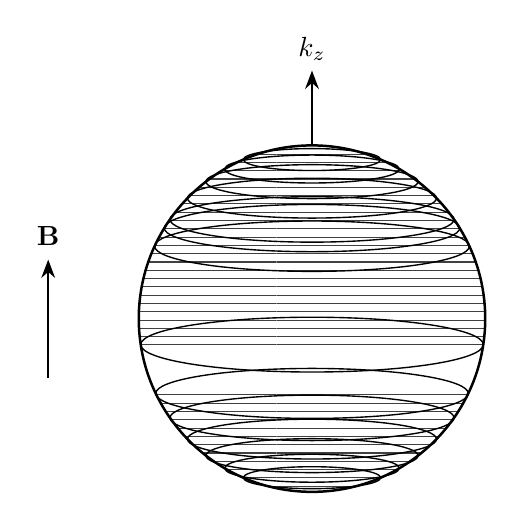
\begin{tikzpicture}[line width=0.8pt,>=Stealth]
% 球体（R=2.2，横向细线填充 = 密集朗道管带）
\fill[pattern=horizontal lines,pattern color=black!75] (0,0) circle (2.2);
% 中腰部偏下一条加宽空白管带
\begin{scope}
  \clip (0,0) circle (2.2);
  \fill[white] (-2.3,-0.95) -- (2.3,-0.95) -- (2.3,-0.33) -- (-2.3,-0.33) -- cycle;
\end{scope}
% 纬向椭圆（朗道管与球面相截的环带边沿；近两极密集，空白管带内不画）
\foreach \y in {2.02,1.9,1.74,1.53,1.26,0.92,1.15}{
  \draw[line width=0.5pt]
    (0,\y) ellipse ({sqrt(4.84-\y*\y)} and {0.16*sqrt(4.84-\y*\y)});
}
\foreach \y in {2.02,1.9,1.74,1.53,1.26}{
  \draw[line width=0.5pt]
    (0,-\y) ellipse ({sqrt(4.84-\y*\y)} and {0.16*sqrt(4.84-\y*\y)});
}
% 空白管带上下边沿
\draw[line width=0.5pt] (0,-0.33) ellipse ({sqrt(4.84-0.33*0.33)} and {0.16*sqrt(4.84-0.33*0.33)});
\draw[line width=0.5pt] (0,-0.95) ellipse ({sqrt(4.84-0.95*0.95)} and {0.16*sqrt(4.84-0.95*0.95)});
% 球轮廓
\draw[line width=0.9pt] (0,0) circle (2.2);
% 顶部 k_z 轴
\draw[->] (0,2.2) -- (0,3.15) node[above] {$k_z$};
% 左侧 B 箭头（向上）
\draw[->] (-3.35,-0.75) -- (-3.35,0.75);
\node[above] at (-3.35,0.8) {$\mathbf{B}$};
\end{tikzpicture}
\end{document}
